\section{Procedimiento}

\subsection{Pedir el MicroROS robot de equilibrio}

Pedir el robot en el enlace de la plataforma del almacén: \url{http://168.176.26.64/proyects/LDIEE/index.php}

\begin{figure}[H]
    \centering
    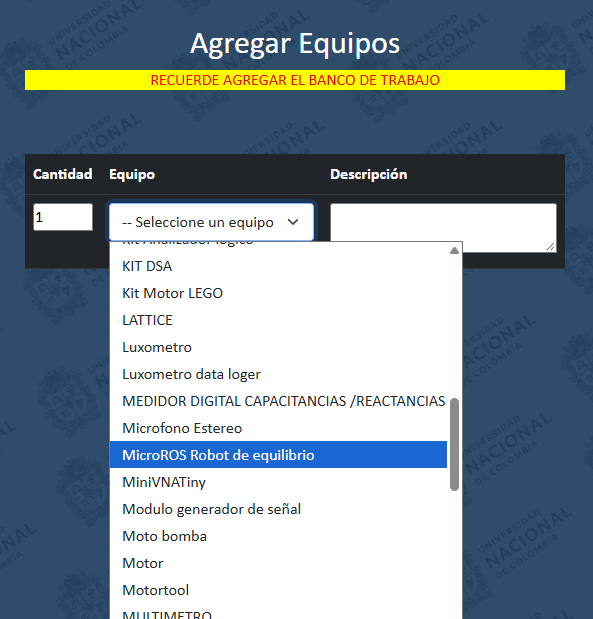
\includegraphics[width=0.5\textwidth]{Images/pedir_MicroROS.png}
    \caption{Plataforma del almacén para solicitar el robot.}
    \label{fig:pedir_microros}
\end{figure}

\subsection{Instalar Visual Studio Code}

\begin{figure}[H]
    \centering
    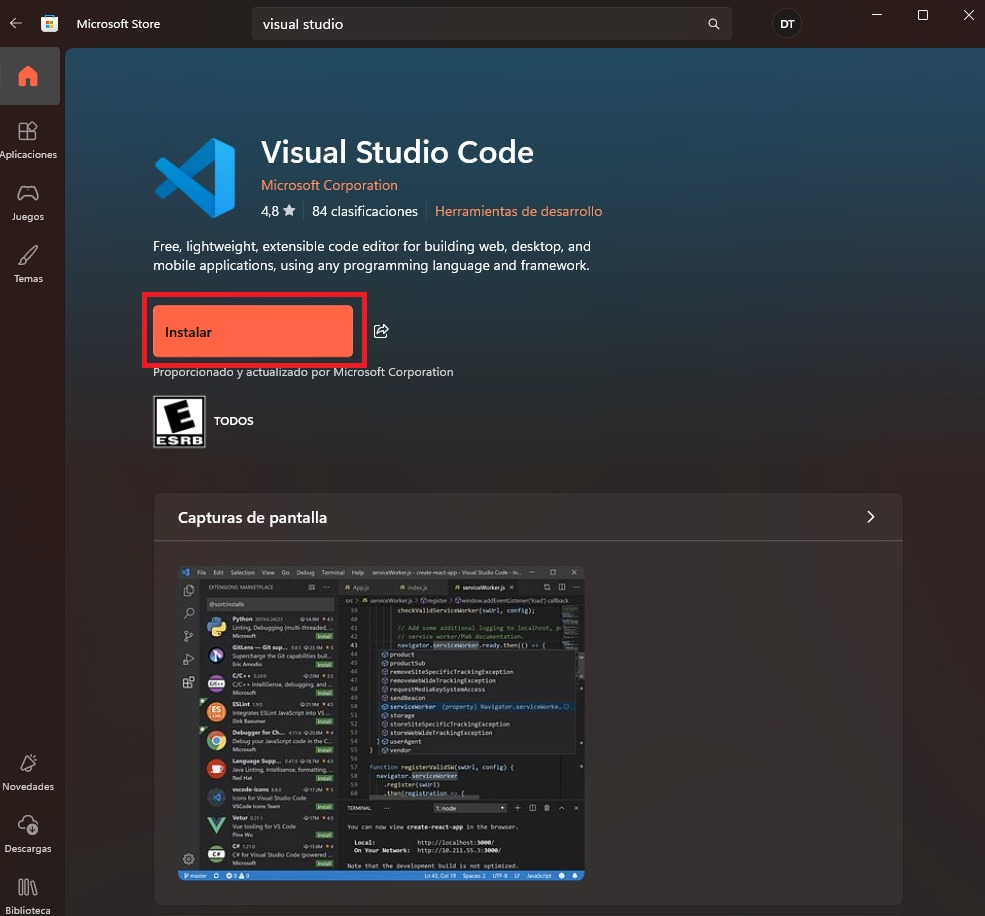
\includegraphics[width=0.4\textwidth]{Images/visual_studio_code.jpeg}
    \caption{Entorno de desarrollo Visual Studio Code.}
    \label{fig:vscode_install}
\end{figure}

\subsection{Instalar la extensión Arm Keil Studio Pack (MDK v6)}

\begin{figure}[H]
    \centering
    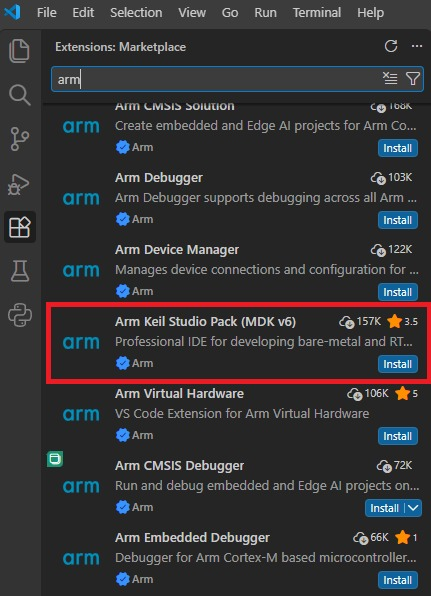
\includegraphics[width=0.4\textwidth]{Images/extension_ARM.jpeg}
    \caption{Extensión Arm Keil Studio Pack en VS Code.}
    \label{fig:extension_arm}
\end{figure}

\subsection{Activar la licencia MDK-Community edition}

En el teclado presionar el atajo \textbf{Ctrl + Shift + P} y seleccionar la opción \textbf{Arm Tools: Manage Arm Tool Licenses} en la pestaña emergente.

\begin{figure}[H]
    \centering
    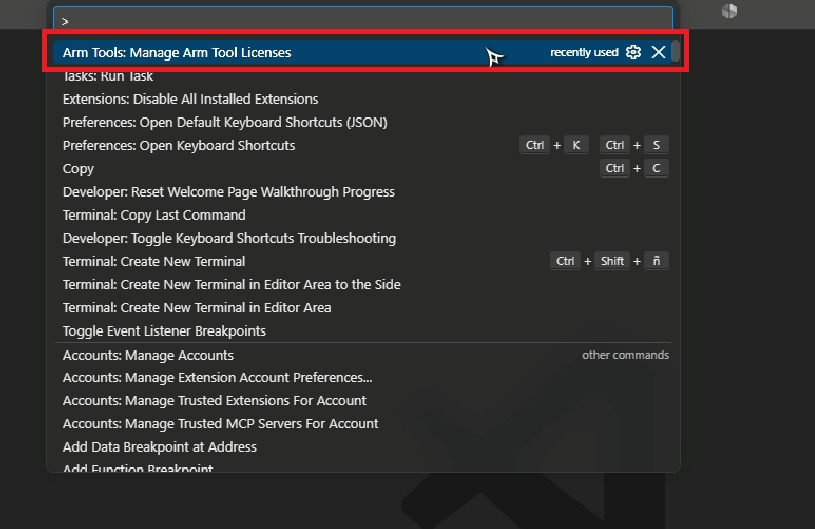
\includegraphics[width=0.5\textwidth]{Images/licencia1.jpeg}
    \caption{Gestión de licencias en Arm Tools.}
    \label{fig:licencia1}
\end{figure}

En la ventana emergente seguir el procedimiento como se indica:

\begin{enumerate}
    \item Seleccionar la opción \textbf{License Server}.
    \item En el espacio de texto pegar el siguiente enlace: \url{https://mdk-preview.keil.arm.com}
    \item Seleccionar el botón \textbf{Query}.
\end{enumerate}

\begin{figure}[H]
    \centering
    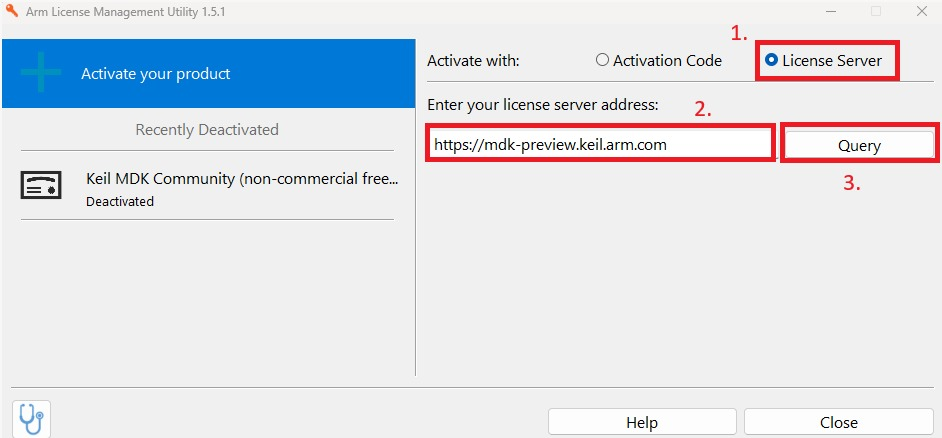
\includegraphics[width=0.7\textwidth]{Images/licencia2.png}
    \caption{Configuración del servidor de licencias.}
    \label{fig:licencia2}
\end{figure}

A continuación, seleccionar el botón \textbf{Activate}.

\begin{figure}[H]
    \centering
    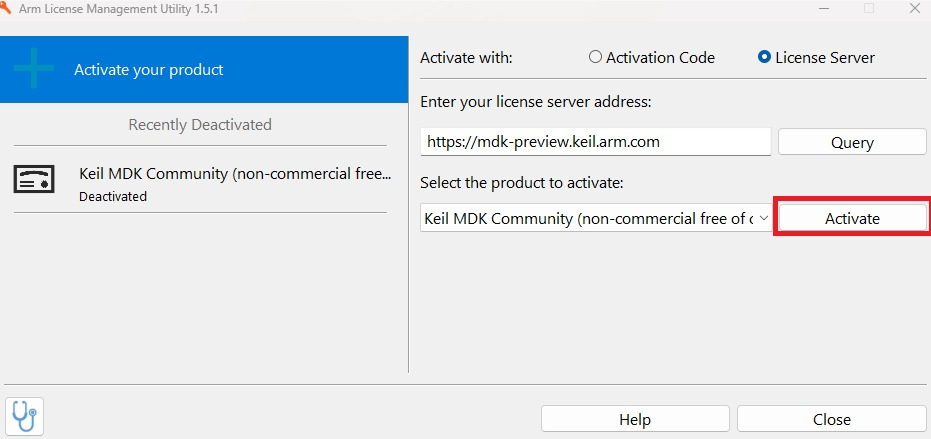
\includegraphics[width=0.7\textwidth]{Images/licencia3.png}
    \caption{Activación de la licencia MDK.}
    \label{fig:licencia3}
\end{figure}

Y por último, seleccionar el botón \textbf{Close}.

\begin{figure}[H]
    \centering
    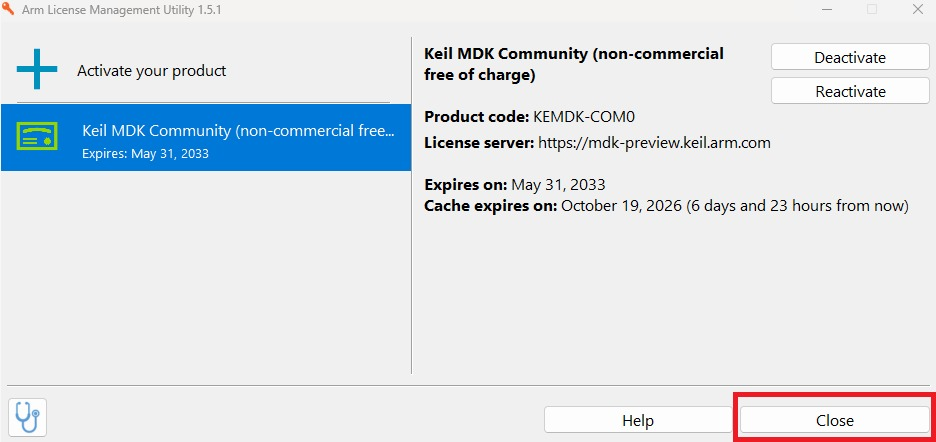
\includegraphics[width=0.7\textwidth]{Images/licencia4.png}
    \caption{Licencia activada con éxito.}
    \label{fig:licencia4}
\end{figure}

\subsection{Descargar el proyecto de control LQR y Drivers}

El código del proyecto se encuentra en el repositorio de GitHub \url{https://github.com/nebisman/RobotPIR}. Para descargarlo como un archivo comprimido (\texttt{.zip}) no es necesario tener una cuenta de GitHub ni instalar Git; basta con seguir estos pasos:

\begin{enumerate}
    \item Abrir en el navegador el enlace del repositorio: \url{https://github.com/nebisman/RobotPIR}.
    \item En la parte superior derecha de la lista de archivos, hacer clic en el botón verde \textbf{Code}.
    \item En el menú desplegable, seleccionar la opción \textbf{Download ZIP} (ubicada al final del menú). El navegador descargará el archivo \texttt{RobotPIR-main.zip}.
    \item Mover el archivo descargado a una ruta corta y sin espacios ni caracteres especiales (por ejemplo, \texttt{C:\textbackslash control}).
    \item Descomprimir el archivo.
    \item Verificar que la carpeta descomprimida contenga las subcarpetas \texttt{APP}, \texttt{BSP}, \texttt{CMSIS}, \texttt{FWLib} y \texttt{USER}. La carpeta \texttt{USER} es la que se abrirá en VS Code en la siguiente sección.
\end{enumerate}

Asimismo, asegúrese de instalar (en caso de ser necesario) el controlador del conversor USB-Serial CH340 \href{https://drive.google.com/drive/folders/1o3UUpWzaBw51vPLUIvo3fhqEAZbRiucU}{adjunto aqui.}

onibles en el siguiente enlace: \url{https://tinyurl.com/mp9cnfty}


\subsection{Abrir la subcarpeta USER del proyecto en VS Code}

Abrir Visual Studio Code y en el menú \textbf{File} seleccionar la opción \textbf{Open Folder}.

\begin{figure}[H]
    \centering
    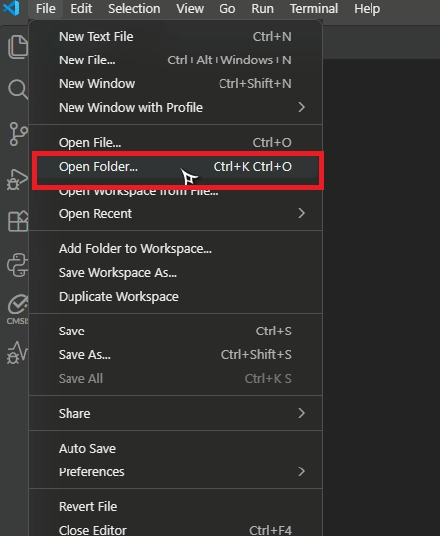
\includegraphics[width=0.5\textwidth]{Images/abrir_lqr1.png}
    \caption{Opción Abrir Carpeta en VS Code.}
    \label{fig:abrir_lqr1}
\end{figure}

Abrir la subcarpeta \textbf{USER} del proyecto \textbf{STM3\_code}. La ruta exacta es:

\[ 
\text{STM32\_code} \rightarrow \text{STM32\_code} \rightarrow \text{USER}
\]

\begin{figure}[H]
    \centering
    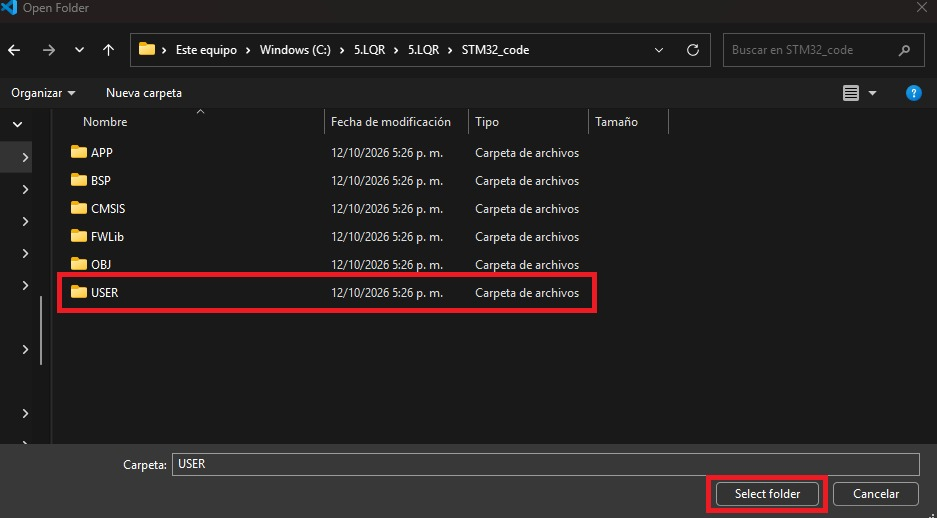
\includegraphics[width=0.7\textwidth]{Images/abrir_lqr2.png}
    \caption{Navegación hasta la subcarpeta USER.}
    \label{fig:abrir_lqr2}
\end{figure}

Ahora, se debe desactivar el modo restringido. En la esquina inferior izquierda de VS Code, seleccionar la opción \textbf{Restricted mode}.

\begin{figure}[H]
    \centering
    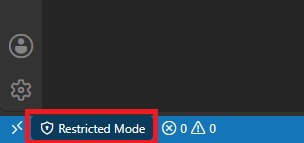
\includegraphics[width=0.7\textwidth]{Images/modo_restringido.png}
    \caption{Indicador de modo restringido.}
    \label{fig:modo_restringido}
\end{figure}

En la ventana emergente, seleccionar el botón \textbf{Trust}.

\begin{figure}[H]
    \centering
    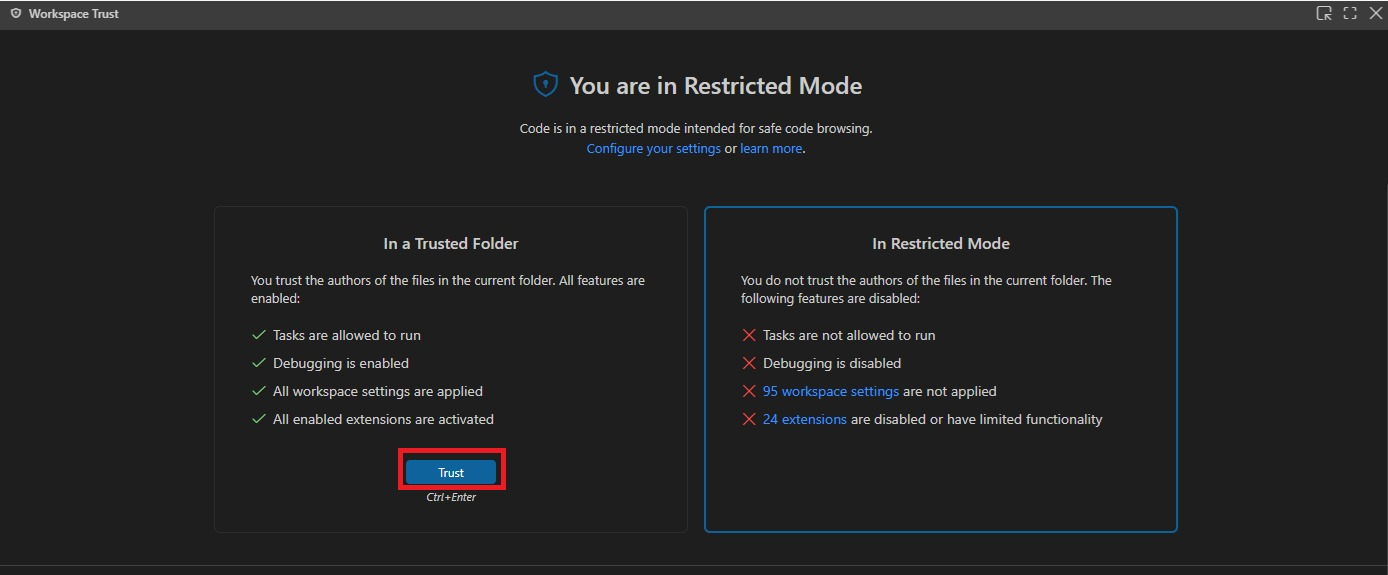
\includegraphics[width=0.7\textwidth]{Images/modo_restringido1.png}
    \caption{Confirmación de confianza en el espacio de trabajo.}
    \label{fig:modo_restringido1}
\end{figure}

\subsection{Construir el proyecto}

Una vez en la carpeta USER, identifique y abra el archivo \texttt{asignacion\_polos.jl} (si va a diseñar un control usando asignación de polos) o \texttt{control\_lqr.jl} (si va a diseñar un control por LQR). Después de abrir el archivo, conecte la tarjeta STM32 del Robot a un puerto serial de su computadora por medio de un cable USB-C. A continuación, oprima el boton de triangulo $\triangleright$ (o elija todo el código con el raton y digite el comando Alt + Enter) y espere a que se compile el proyecto y se flashee la STM32 (de ser necesario, instale los paquetes que se requieran en la terminal). Si esta parte se desarrollo correctamente, se mostrará el siguiente mensaje.

\begin{figure}[H]
    \centering
    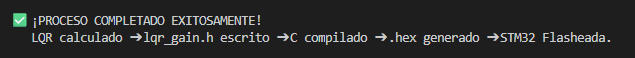
\includegraphics[width=0.7\textwidth]{Images/exito.png}
    \caption{Desarrollo exitoso de la compilación y flasheo.}
    \label{fig:exito}
\end{figure}

\subsection{Encender y probar el robot}
\label{sec:encender}

Una vez cargado el programa:
\begin{enumerate}
    \item Desconectar el cable USB-C del robot.
    \item Activar el switch de encendido para alimentar la tarjeta mediante las baterías.
    \item Posicionar el robot de forma vertical sobre una superficie de prueba.
    \item Presionar y soltar el botón \textbf{RESET}, esperar un segundo y presionar el botón \textbf{KEY1} para iniciar el control de equilibrio.
\end{enumerate}
